\documentclass[rusmathsym, eqnumwithinsec, amspack, hyperref]{bomgost}

\DeclareTextSymbol{\CYRA}\UnicodeEncodingName{"0410}        % А
\DeclareTextSymbol{\cyra}\UnicodeEncodingName{"0430}        % а
\DeclareTextSymbol{\CYRB}\UnicodeEncodingName{"0411}        % Б
\DeclareTextSymbol{\cyrb}\UnicodeEncodingName{"0431}        % б
\DeclareTextSymbol{\CYRV}\UnicodeEncodingName{"0412}        % В 
\DeclareTextSymbol{\cyrv}\UnicodeEncodingName{"0432}        % в
\DeclareTextSymbol{\CYRG}\UnicodeEncodingName{"0413}        % Г
\DeclareTextSymbol{\cyrg}\UnicodeEncodingName{"0433}        % г
\DeclareTextSymbol{\CYRD}\UnicodeEncodingName{"0414}        % Д
\DeclareTextSymbol{\cyrd}\UnicodeEncodingName{"0434}        % д
\DeclareTextSymbol{\CYRE}\UnicodeEncodingName{"0415}        % Е 
\DeclareTextSymbol{\cyre}\UnicodeEncodingName{"0435}        % е
\DeclareTextSymbol{\CYRZH}\UnicodeEncodingName{"0416}       % Ж 
\DeclareTextSymbol{\cyrzh}\UnicodeEncodingName{"0436}       % ж
\DeclareTextSymbol{\CYRZ}\UnicodeEncodingName{"0417}        % З
\DeclareTextSymbol{\cyrz}\UnicodeEncodingName{"0437}        % з
\DeclareTextSymbol{\CYRI}\UnicodeEncodingName{"0418}        % И
\DeclareTextSymbol{\cyri}\UnicodeEncodingName{"0438}        % и
\DeclareTextSymbol{\CYRISHRT}\UnicodeEncodingName{"0419}    % Й
\DeclareTextSymbol{\cyrishrt}\UnicodeEncodingName{"0439}    % й
\DeclareTextSymbol{\CYRK}\UnicodeEncodingName{"041A}        % К
\DeclareTextSymbol{\cyrk}\UnicodeEncodingName{"043A}        % к
\DeclareTextSymbol{\CYRL}\UnicodeEncodingName{"041B}        % Л
\DeclareTextSymbol{\cyrl}\UnicodeEncodingName{"043B}        % л 
\DeclareTextSymbol{\CYRM}\UnicodeEncodingName{"041C}        % М
\DeclareTextSymbol{\cyrm}\UnicodeEncodingName{"043C}        % м
\DeclareTextSymbol{\CYRN}\UnicodeEncodingName{"041D}        % Н
\DeclareTextSymbol{\cyrn}\UnicodeEncodingName{"043D}        % н
\DeclareTextSymbol{\CYRO}\UnicodeEncodingName{"041E}        % О
\DeclareTextSymbol{\cyro}\UnicodeEncodingName{"043E}        % о
\DeclareTextSymbol{\CYRP}\UnicodeEncodingName{"041F}        % П
\DeclareTextSymbol{\cyrp}\UnicodeEncodingName{"043F}        % п
\DeclareTextSymbol{\CYRR}\UnicodeEncodingName{"0420}        % Р
\DeclareTextSymbol{\cyrr}\UnicodeEncodingName{"0440}        % р
\DeclareTextSymbol{\CYRS}\UnicodeEncodingName{"0421}        % С
\DeclareTextSymbol{\cyrs}\UnicodeEncodingName{"0441}        % с
\DeclareTextSymbol{\CYRT}\UnicodeEncodingName{"0422}        % Т
\DeclareTextSymbol{\cyrt}\UnicodeEncodingName{"0442}        % т
\DeclareTextSymbol{\CYRU}\UnicodeEncodingName{"0423}        % У
\DeclareTextSymbol{\cyru}\UnicodeEncodingName{"0443}        % у
\DeclareTextSymbol{\CYRF}\UnicodeEncodingName{"0424}        % Ф
\DeclareTextSymbol{\cyrf}\UnicodeEncodingName{"0444}        % ф
\DeclareTextSymbol{\CYRH}\UnicodeEncodingName{"0425}        % Х
\DeclareTextSymbol{\cyrh}\UnicodeEncodingName{"0445}        % х
\DeclareTextSymbol{\CYRC}\UnicodeEncodingName{"0426}        % Ц
\DeclareTextSymbol{\cyrc}\UnicodeEncodingName{"0446}        % ц
\DeclareTextSymbol{\CYRCH}\UnicodeEncodingName{"0427}       % Ч
\DeclareTextSymbol{\cyrch}\UnicodeEncodingName{"0447}       % ч
\DeclareTextSymbol{\CYRSH}\UnicodeEncodingName{"0428}       % Ш
\DeclareTextSymbol{\cyrsh}\UnicodeEncodingName{"0448}       % ш
\DeclareTextSymbol{\CYRSHCH}\UnicodeEncodingName{"0429}     % Щ
\DeclareTextSymbol{\cyrshch}\UnicodeEncodingName{"0449}     % щ
\DeclareTextSymbol{\CYRHRDSN}\UnicodeEncodingName{"042A}    % Ъ
\DeclareTextSymbol{\cyrhrdsn}\UnicodeEncodingName{"044A}    % ъ
\DeclareTextSymbol{\CYRERY}\UnicodeEncodingName{"042B}      % Ы
\DeclareTextSymbol{\cyrery}\UnicodeEncodingName{"044B}      % ы
\DeclareTextSymbol{\CYRSFTSN}\UnicodeEncodingName{"042C}    % Ь
\DeclareTextSymbol{\cyrsftsn}\UnicodeEncodingName{"044C}    % ь
\DeclareTextSymbol{\CYREREV}\UnicodeEncodingName{"042D}     % Э
\DeclareTextSymbol{\cyrerev}\UnicodeEncodingName{"044D}     % э
\DeclareTextSymbol{\CYRYU}\UnicodeEncodingName{"042E}       % Ю
\DeclareTextSymbol{\cyryu}\UnicodeEncodingName{"044E}       % ю
\DeclareTextSymbol{\CYRYA}\UnicodeEncodingName{"042F}       % Я
\DeclareTextSymbol{\cyrya}\UnicodeEncodingName{"044F}       % я

% Закомментируйте это, если hyperref не нужен. 
% Изменение уровня \subparagraph (приложения) в закладках pdf документа. 
% Это нужно для сохранения правильной иерархии закладок в pdf документе.
\makeatletter%
\renewcommand{\toclevel@subparagraph}{2}%
\makeatother% 

% Для вставки программного кода.
\usepackage{listings}

% "Умная" запятая: \(0,2\) - число, \(0, 2\) - перечисление.
\usepackage{icomma}
\usepackage{float}
\usepackage{pgfplots}
\usepackage{pgfplotstable}
\usepackage{longtable}
\usepackage{cleveref}


\pgfplotsset{compat=newest}

\pgfplotstableset{set thousands separator={}, precision=3, use comma, col sep=comma, header=true,
every head row/.style={before row=\hline, after row=\hline},
every even row/.style={after row=\hline},
every odd row/.style={after row=\hline},
every column/.style={column type/.add={|}{}},
every last column/.style={column type/.add={}{|}},
columns/text/.style={string type},
}

\author{Кухта А.В.}
\title{Разработка устройства для калибровки для исследования характеристик антенно-фидерного и приёмного тракта иркутского радара}
\date{\today}


\begin{document}

\maketitle
\thispagestyle{empty}
\newpage

\begin{abstract}
% Для добавления общего числа приложений нужно добавить команду \printtotapp[.]
% Во всех командах существует необязательный аргумент, который добавляется в конец команды. По умолчанию это запятая. Это нужно для случаев, когда каких-то элементов в работе нет т. е. их счётчики равны 0. В этом случае команда ничего не выведет. Так как порядок команд может быть любым и необходимо, чтобы после последней команды была точка, а между командами запятая, поэтому добавлен необязательный аргумент.
Курсовая работа содержит \printtotpage \printtotfig \printtottab \printtotref[.] В~некоторых случаях количество приложений не указывается. 

% Для количества приложений команда аналогична: \total{totappendix}~приложений.

КЛЮЧЕВОЕ СЛОВО~1, КЛЮЧЕВОЕ СЛОВО~2, КЛЮЧЕВОЕ СЛОВО~3 и т. д.

Краткое описание работы.
\end{abstract}


\tableofcontents


\section*{ОБОЗНАЧЕНИЯ И СОКРАЩЕНИЯ}
fff

%
% ВВЕДЕНИЕ
%

\section*{ВВЕДЕНИЕ}
Исследования процессов, происходящих в верхней части атмосферы Земли, ионосфере и окружающем космическом пространстве является важной научной задачей в понимании физики процессов в системе Солнце-Земля.

Одними из наиболее информативных научных инструментов в этих исследованиях являются радары некогерентного рассеяния. Это очень мощные и дорогостоящие установки, которых в мире насчитывается около 10 штук. Одним из таких радаров является единственный в России Иркутский радар некогерентного рассеяния (ИРНР).

ИРНР является уникальным инструментом. Он используется для изучения процессов, происходящих в атмосфере Земли, наблюдения за звездными радиоисточниками, а также для экспериментов по обнаружению и сопровождению космических объектов.

Ниже представлены ключевые характеристики ИРНР из источника \cite{Kushnarev}:

\begin{itemize}
	\item Диапазон рабочих частот: 154--162 МГц.
	\item Пиковая мощность, достигаемая на двух передатчиках: 2.8 МВт.
	\item Длительность зондирующего импульса: от 70 до 900 мкс.
	\item Частота следования импульса: 24.4 Гц.
	\item Коэффициент усиления антенны: около 35 дБ.
\end{itemize}

ИРНР является радиолокационной станцией и во всех экспериментах крайне важно знать параметры всего приемо-передающего тракта, учитывать его задержки и нестабильность. Например, когда ИРНР работает в режиме наблюдения за космическими объектами, он использует задержку возвращения сигнала для определения расстояния до объекта. Для объектов на высоте 400 км, эта задержка составляет примерно 2600 мкс, и погрешность в одну микросекунду внесёт ~150 метров неточности в определённое расстояние. Следовательно, до проведения экспериментов необходимо измерить и учесть все собственные задержки оборудования ИРНР и компенсировать их в дальнейшем.

Для решения этой задачи необходимо создать генератор тестовых сигналов (калибратор). Он будет формировать сигналы с известными параметрами (длительность импульса, частота, задержка, уровень амплитуды, модуляция) и позволит измерить собственные задержки оборудования, нестабильность характеристик каналов приёма, разность фаз между каналами, а также АЧХ и ФЧХ всего приемного тракта ИРНР.

Требования к генератору сигналов:

\begin{itemize}
	\item Возможность формирования сигналов на рабочих частотах ИРНР: 154--162 МГц.
	\item Длительность импульсов: от 100 до 1000 мкс.
	\item Заданная задержка для импульсов: от 150 до 10000 мкс.
	\item Возможность установки произвольных уровней амплитуды.
	\item Возможность формирования сигналов с линейной частотной модуляцией.
	\item Возможность формирования сигналов с фазовой манипуляцией.
	\item Управление: по Ethernet или USB.
\end{itemize}

Для реализации такого генератора было выбрано следующее оборудование:

\begin{itemize}
	\item Отладочная плата NUCLEO-F746ZG на основе микроконтроллера STM32.
	\item Отладочная плата синтезатора частот на основе чипа AD9910.
\end{itemize}

Выбор именно этих компонентов (отладочная плата Nucleo и синтезатор AD9910) был обусловлен уже имеющимися требованиями. Задача работы состоит в согласовании микроконтроллера и синтезатора частот, разработке алгоритмов управления и создании программного обеспечения (ПО) для микроконтроллера, реализующего все требования к генератору.



\mainpart


\section{ТЕОРЕТИЧЕСКАЯ ЧАСТЬ}
\subsection{Цифровые синтезаторы частот}

Цифровые синтезаторы частот, также известные как DDS (Direct Digital Synthesizer), являются классом устройств, которые предназначены для создания сигнала с настраиваемой частотой, фазой и амплитудой.

DDS используются:

\begin{itemize}
	\item В качестве источников тактовой частоты в тех задачах, где требуется изменение тактовой частоты в реальном времени.
	\item В качестве модуляторов для передачи данных.
	\item В атомных интерферометрах.
	\item В радарах.
\end{itemize}

Главными внутренними компонентами DDS являются:

\begin{itemize}
	\item Аккумулятор фазы, от разрядности которого (напр. 24, 32 или 48 бит) зависит точность выбора частоты сигнала.
	\item Блок конверсии фазы в амплитуду.
	\item Цифро-аналоговый преобразователь (ЦАП), разрешение которого влияет на точность реконструкции аналогового сигнала.
\end{itemize}

Принцип работы DDS заключается в цикличном добавлении кода частоты (Frequency Tuning Word, FTW) к аккумулятору фазы с последующим преобразованием фазы в амплитуду, при помощи таблицы или алгоритма аппроксимации. Для управления фазой после аккумулятора фазы добавляется блок сдвига фазы, который добавляет код смещения фазы к изначальному значению фазы. Для управления амплитудой после блока конверсии фазы в амплитуду добавляется блок масштабирования амплитуды, который уменьшает амплитуду на заданный коэффициент. Значения амплитуды затем поступают на ЦАП и преобразуются в аналоговый сигнал.

Помимо разрешения аккумулятора фазы и ЦАП, важной характеристикой любого DDS также является максимальная внутренняя частота, от которой зависит максимальная синтезируемая частота.

Углублённое описание принципов работы DDS можно найти в источнике \cite{DDSIntro}, а детальное рассмотрение некоторых особенностей синтезируемых при помощи DDS сигналов можно найти в источнике \cite{DDSTutorial}.

\subsection{Формирование сигналов}

Использование калибратора предполагается в сочетании как с аналоговыми блоками приёма и фильтрации ИРНР, так и с регистрирующим оборудованием ИРНР (АЦП, цифровая обработка сигналов и т.д.).

Задача калибратора состоит в том, чтобы создавать сигналы заранее известной формы, которые проходя через все блоки приема ИРНР регистрируются в виде цифровых отсчетов в штатном регистрирующем оборудовании ИРНР.

Прохождение сигнала через цепочки оборудования ИРНР может исказить его --- под искажением понимается любое изменение сигнала --- и это искажение требуется характеризовать.

Искажения можно выразить через амплитудно-частотную характеристику (АЧХ) и фазово-частотную характеристику (ФЧХ).

Амплитудно-частотная характеристика описывает уровень амплитуды в зависимости от частоты после прохождения через среду и отражает затухание разных частот.

\subsection{Спектральный анализ}

Имея запись некоторого сигнала, можно найти количество некоторой частотной составляющей в нём, вычислив сумму произведений этого сигнала и сигнала, полностью заполненного сигналом интересующей частоты. Это работает, так как:

% https://tex.stackexchange.com/questions/47170/how-to-write-conditional-equations-with-one-sided-curly-brackets
\begin{equation}
	\int_{-\infty}^{\infty}{\sin(ax)\sin(bx)}{dx}
	\begin{cases}
		\infty,& a = b\\
		0,     & a \neq b
	\end{cases}
\end{equation}

Можно проверить, что это действительно так, при помощи небольшой программы на Python с использованием библиотеки numpy, которая вычисляет сумму произведений двух сигналов, для случая с сигналами одинаковой частоты и разной частоты:

% https://tex.stackexchange.com/questions/106770/how-to-add-line-numbers-to-a-program-listing-code
% https://tex.stackexchange.com/questions/50107/adjust-bottom-margin-of-a-listing-environment
\lstset{
	language=c,
	basicstyle=\scriptsize\ttfamily,
	numbers=left,
	stepnumber=1,
	showstringspaces=false,
	tabsize=4,
	breaklines=true,
	breakatwhitespace=false,
	xleftmargin=.1\textwidth, xrightmargin=.1\textwidth,
	belowskip=1em, aboveskip=1em
}
\begin{lstlisting}
import numpy as np

x = np.arange(1000)

print( np.sin(x) @ np.sin(x) )   # 499.5
print( np.sin(x) @ np.sin(2*x) ) # -0.01
\end{lstlisting}

В приведённом выше примере рассматривается случай с извлечением составляющих с известной частотой и известной начальной фазой, то есть сигналы вида $\sin(x+0)$. Если же начальная фаза не известна, как часто бывает на практике, то её можно извлечь исходя из следующего:

\begin{equation}
	\int_{-\infty}^{\infty}{\sin(x)\cos(x)}{dx}=0
\end{equation}

А также формулы суммы тригонометрических функций, когда, например, $\sin(x+2)$ на самом деле является $\cos(2)\sin(x) + \sin(2)\cos(x)$, или примерно $-0.416\sin(x) + 0.909\cos(x)$

% TODO: DDS
% TODO: Модуляция
% TODO: ЛЧМ
% TODO: AD9910 аппроксимирует ЛЧМ сигналы при помощи дискретных шагов по частоте.

%
% Практическая часть
%
\section{ПРАКТИЧЕСКАЯ ЧАСТЬ}
\subsection{Описание устройства}

Калибратор представляет собой генератор сигналов, предназначенный для подачи коротких сигналов (импульсов) по внешнему событию (триггеру) с возможностью настройки параметров сигналов и задания последовательностей сигналов с разными параметрами.

В состав калибратора входят: отладочная плата AD9910 PCBZ с синтезатором и отладочная плата Nucleo F746ZG с микроконтроллером, а также мезонинная плата, которая выводит необходимые управляющие сигналы с микроконтроллера и предоставляет необходимые напряжения питания.

Ниже представлено схематичное изображение калибратора:

%
% Блок-схема устройства
%
\begin{gostfigure}
\begin{figure}[H]
\centering
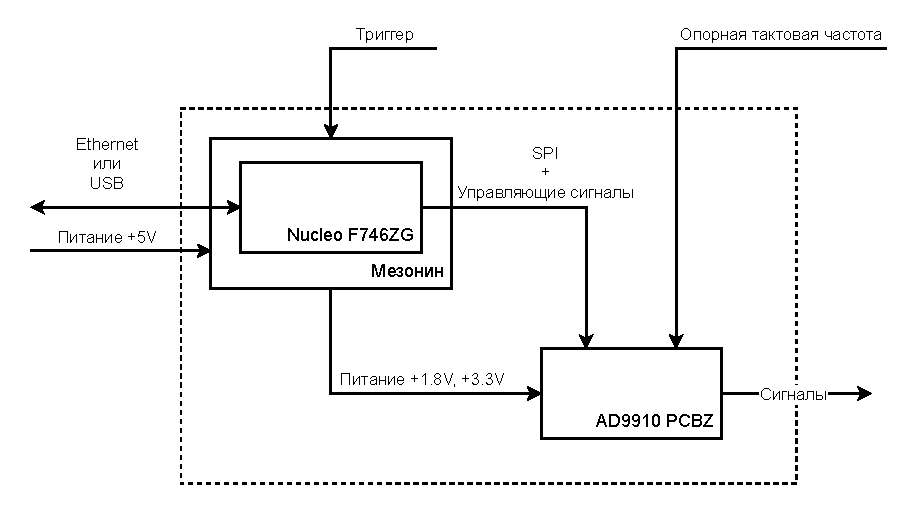
\includegraphics{data/system_architecture.drawio.pdf}
\caption{Общая схема калибратора.}
\label{fig:system_architecture}
\end{figure}
\end{gostfigure}

Управление калибратором осуществляется c ПК по USB или Ethernet, через виртуальный ком-порт в первом случае и через утилиту netcat во втором случае. Калибратор предоставляет текстовый интерфейс, который включает в себя команды добавления сигналов в очередь, очистки очереди, запуска и остановки воспроизведения из очереди.

\pagebreak

Триггерный сигнал может предоставляться как внешним оборудованием ИРНР, так и самим микроконтроллером: на мезонинной плате предусмотрена перемычка, которая позволяет выбирать внешний либо внутренний источник. Частота следования сигналов триггера может варьироваться в разумных пределах; внутренний источник сконфигурирован под стробирующий сигнал с частотой 25 Гц.

Ниже представлено схематичное изображение процесса подачи сигналов, схожее с тем, что можно было бы увидеть на осциллографе:

%
% Схематичное изображение процесса работы
%
\begin{gostfigure}
\begin{figure}[H]
\centering
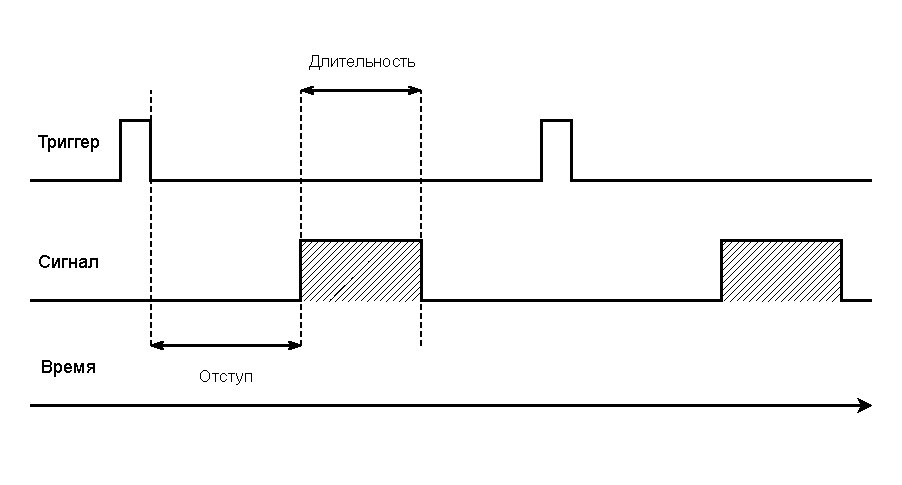
\includegraphics{data/timing_diagram.drawio.pdf}
\caption{Временная схема сигналов.}
\label{fig:timing_diagram}
\end{figure}
\end{gostfigure}

\subsection{Выбор инструментов}

Прошивка для микроконтроллера написана на языке программирования C, с использованием преимущественно свободных инструментов с открытым исходным кодом.

В качестве компилятора C использован gcc для ARM; все используемые в проекте библиотеки нацелены именно на этот компилятор, что и послужило главной причиной для его выбора. Возможной альтернативой является компилятор clang в составе проекта LLVM, но не проверялось, сможет ли он без ошибок собрать все задействованные библиотеки, в особенности STM32 HAL, который может содержать специфичный для gcc код.

В качестве системы сборки использован GNU Make. Задача Make состоит в запуске команд сборки, также называемых правилами, для каждого файла с исходным кодом. Главное преимущество от использования Make по сравнению с, например, скриптом сборки для интерпретатора командной строки, будь это bash или что-нибудь другое, заключается в возможности параллельной сборки, когда не зависящие друг от друга файлы с исходным кодом собираются параллельно, что позволяет существенно ускорить полную сборку проекта. Другим преимуществом является поддержка частичной сборки, когда повторно компилируются только файлы, изменившиеся с момента предыдущей сборки. Нужно отметить, что существуют и другие системы сборки, например CMake и ninja, которые обладают схожими возможностями, но часто сложнее в использовании.

В качестве IDE использована среда разработки VSCode, которая была выбрана преимущественно в связи с её популярностью и наличием расширения C/C++ IntelliSense, которое предоставляет быстрый поиск идентификаторов во всех файлах проекта и является незаменимым инструментом при изучении кода больших библиотек, таких как STM32 HAL. Нужно отметить, что, в отличие от самого VSCode, это расширение не является полностью свободным --- его исходный код закрыт. Другими IDE, которе бы подошли для разработки прошивки под ARM устройство, являются Qt Creator и CLion.

В качестве инструмента для загрузки собранной прошивки в микроконтроллер и отладки использован OpenOCD. Этот инструмент позволяет прошивать множество микроконтроллеров от разных производителей, а также выступает сервером отладки для gdb.

Наконец, в качестве отладчика использован gdb, который не имеет возможности самостоятельно взаимодействовать с отлаживаемым устройством и полагается на OpenOCD в качестве сервера.

\subsection{Использование STM32}

\subsubsection{Технические характеристики}

В данной работе используется отладочная макетная плата NUCLEO-F746ZG с микроконтроллером STM32F746ZG, системой питания, отладчиком ST-LINK и вспомогательной периферией (кнопки, порты, и т.д.). Микроконтроллер STM32F746ZF является системой на чипе и включает в себя процессорное ядро, оперативную память, флеш память, связующие шины и набор аппаратных блоков фиксированной функции, таких как таймеры и разнообразные интерфейсы. Наиболее важные характеристики микроконтроллера представлены ниже:

\begin{itemize}
	\item Ядро ARM Cortex-M7, оснащённое 4 КБ кэша инструкций и данных, работающее на частоте от 16 МГц до 216 МГц.
	\item Интерфейс SWD, позволяющий производить детальную отладку с компьютера, включая просмотр памяти и содержимого регистров процессора, а также добавление точек остановки на отдельные инструкции.
	\item 320 КБ внутренней оперативной памяти. Для решения более требовательных к памяти задач контроллер памяти предусматривает возможность добавления внешней оперативной памяти.
	\item 1 МБ внутренней флэш-памяти для хранения кода и данных прошивки. Возможно добавление до 256 МБ внешней флэш-памяти при помощи интерфейса QSPI.
	\item Доступно вплоть до 168 GPIO, в зависимости от корпуса чипа и настроек интерфейсов.
	\item Множество периферийных интерфейсов, таких как SPI, UART, I2C, PWM, таймеры и др.
\end{itemize}

Более полные характеристики этого чипа можно найти в источнике \cite{STM32F746Datasheet}.

Макетная плата Nucleo примечательна следующим:

\begin{itemize}
	\item Встроенный модуль-отладчик, который позволяет питать плату от USB, производить отладку по протоколу ST-LINK v2, отвечает за процесс прошивки и предоставляет микроконтроллеру возможность отправлять и принимать данные с компьютера, выступая мостиком USB--UART.
	\item Ethernet-порт и микросхема PHY LAN8742A для подключения микроконтроллера к локальной сети.
	\item Три программируемых светодиода, которые можно использовать для индикации ошибок или событий.
	\item Гребенки контактов на нижней стороне платы и разъёмы на верхней стороне платы, которые выводят многие (но не все) GPIO с микроконтроллера.
\end{itemize}

Полный список характеристик этой отладочной платы можно найти в источнике \cite{NucleoDatasheet}.

\subsubsection{Компиляция прошивки}

В состав прошивки входят несколько ключевых компонентов:

\begin{itemize}
	\item Библиотека HAL для STM32F7xx, предоставляющая набор абстракций для работы с аппаратным обеспечением микроконтроллера. Распространяемый по лицензии BSD исходный код получен из официального репозитория и расположен в директории STM32CubeF7/ в рамках структуры файлов проекта.
	\item Ядро операционной системы FreeRTOS, реализующее многозадачность. Распространяемый по лицензии MIT исходный код получен из официального репозитория и расположен в директории FreeRTOS-Kernel/ в рамках структуры файлов проекта.
	\item Библиотека FreeRTOS-Plus-TCP с реализацией TCP/IP стека и драйвера для Ethernet-контроллера. Распространяемый по лицензии MIT исходный код получен из официального репозитория и расположен в директории FreeRTOS-Plus-TCP/ в рамках структуры файлов проекта.
	\item Набор дополнений к FreeRTOS, включая реализацию режима сна и аллокатор памяти с возможностью наращивания размера блоков. Построен с нуля или на основе кода других компонентов и расположен в директории freertos\_extras/ в рамках структуры файлов проекта.
	\item Библиотека picolibc в качестве стандартной библиотеки C, реализующей функции printf, scanf, strtod и др. В отличие от всех остальных компонентов, представлена в двоичной форме, а не в виде исходного кода. Расположена в файле libc.a в корневой директории в рамках структуры файлов проекта.
	\item Код приложения, связывающий все вышеперечисленные компоненты и реализующий:
	\begin{itemize}
		\item Инициализацию микроконтроллера.
		\item Текстовый пользовательский интерфейс.
		\item Алгоритмы управления синтезатором AD9910.
	\end{itemize}
\end{itemize}

Данный набор библиотек был получен не сразу. На ранних стадиях разработки использовался только HAL в сочетании с поставляющейся в комплекте с компилятором GCC стандартной библиотекой C newlib-nano, без использования операционной системы FreeRTOS.

Позднее, когда была реализована и проверена базовая логика управления синтезатором и настало время реализовать управление по Ethernet, было добавлено ядро FreeRTOS и библиотека FreeRTOS-Plus-TCP, и код приложения был адаптирован под использование предоставляемых FreeRTOS возможностей.

Наконец, библиотека newlib-nano была заменена библиотекой picolibc из-за неудовлетворительных характеристик предоставляемого в newlib-nano аллокатора памяти, а также отсутствия возможности переопределить функцию printf собственной версией, что требовалось для реализации перенаправления вывода при управлении по Ethernet. Библиотека picolibc не предоставляет аллокатор памяти, вместо этого был использован аллокатор heap5 в составе FreeRTOS, который был модифицирован для добавления поддержки функции realloc.

Процесс сборки прошивки происходит в два этапа: сборка отдельных файлов с исходным кодом (единиц трансляции) в объектные файлы, затем компоновка всех объектных файлов в итоговый бинарный файл с использованием использованием специфичного для микроконтроллера компоновочного скрипта.

Ниже представлен фрагмент файла Makefile, отвечающий за флаги компилятора при сборке и компоновке:

\lstset{
	language=c,
	basicstyle=\scriptsize\ttfamily,
	numbers=left,
	stepnumber=1,
	showstringspaces=false,
	tabsize=4,
	breaklines=true,
	breakatwhitespace=false,
	xleftmargin=.1\textwidth, xrightmargin=.1\textwidth,
	belowskip=1em, aboveskip=1em
}
\begin{lstlisting}
MCU_FLAGS = -mcpu=cortex-m7 -mfpu=fpv4-sp-d16 -mfloat-abi=hard

CC	 = arm-none-eabi-gcc
FLAGS	 = $(MCU_FLAGS) $(DEFINES) $(INCLUDE) -g -c -O2 -Wall -Wextra
LFLAGS	 = $(MCU_FLAGS) -T $(LDSCRIPT) -Wl,--print-memory-usage -Wl,--gc-sections -Wl,-Map=firmware.map,--cref -nostdlib
\end{lstlisting}

Здесь указывается тип процессора, под который требуется генерировать код, а также обозначается наличие аппаратного FPU одинарной точности. Помимо указания типа процессора, использован флаг {\footnotesize\ttfamily{``-g''}} для добавления минимальной отладочной информации и {\footnotesize\ttfamily{``-O2''}} для использования среднего уровня оптимизаций, а также включен набор предупреждений {\footnotesize\ttfamily{``-Wall -Wextra''}} о потенциальных ошибках в коде. Помимо этого, в переменной DEFINES передаётся набор директив препроцессора, необходимых для сборки HAL именно под чип STM32F746, а в переменной INCLUDE передаётся набор директорий для поиска заголовочных файлов.

Ещё один важный флаг компилятора указывается непосредственно в правиле для сборки отдельных файлов с кодом. Данное правило представлено ниже:

\lstset{
	language=c,
	basicstyle=\scriptsize\ttfamily,
	numbers=left,
	stepnumber=1,
	showstringspaces=false,
	tabsize=4,
	breaklines=true,
	breakatwhitespace=false,
	xleftmargin=.1\textwidth, xrightmargin=.1\textwidth,
	belowskip=1em, aboveskip=1em
}
\begin{lstlisting}
%.o: %.c
	@echo " [CC]" $<
	@$(CC) $(FLAGS) -flto -o $@ $<
\end{lstlisting}

Добавляемый здесь флаг {\footnotesize\ttfamily{``-flto''}} включает полнопрограммную оптимизацию, что приводит к заметному уменьшению размеров программы из-за удаления недостижимого кода.

При компоновке, для предотвращения включения в сборку поставляемой с компилятором стандартной библиотеки указывается флаг {\footnotesize\ttfamily{``-nostdlib''}}, а флагом {\footnotesize\ttfamily{``\verb!-Wl,-Map=firmware.map,--cref!''}} включается генерация детального отчёта о источнике каждой функции в итоговом файле, а также добавляется флаг {\footnotesize\ttfamily{``\verb!-Wl,--gc-sections!''}} для удаления незадействованного кода. Помимо этого, добавляется флаг {\footnotesize\ttfamily{``\verb!--Wl,--print-memory-usage!''}} для вывода объёма занятой флеш-памяти и объёма зарезервированной под статические переменные оперативной памяти, в виде короткого отчёта следующего вида по завершении компоновки:

\lstset{
	language=c,
	basicstyle=\scriptsize\ttfamily,
	numbers=left,
	stepnumber=1,
	showstringspaces=false,
	tabsize=4,
	breaklines=true,
	breakatwhitespace=false,
	xleftmargin=.1\textwidth, xrightmargin=.1\textwidth,
	belowskip=1em, aboveskip=1em
}
\begin{lstlisting}
Memory region         Used Size  Region Size  %age Used
             RAM:      100784 B       320 KB     30.76%
           FLASH:      175956 B         1 MB     16.78%
\end{lstlisting}

Размер и адрес регионов FLASH и RAM определён в компоновочном скрипте, путь к которому передан аргументом после флага {\footnotesize\ttfamily{``-T''}}. Помимо размеров памяти, компоновочный скрипт определяет порядок следования различных секций в памяти и предоставляет некоторые адреса в виде переменных, которые доступны в программном коде на C. В частности, компоновочный скрипт предоставляет адреса начала и конца кучи, что используется для инициализации аллокатора.

Ниже представлена таблица секций в порядке их следования в памяти:

% %%%%%%%%%%%%%%%%%%%%%%%
% Таблица секций в памяти
% %%%%%%%%%%%%%%%%%%%%%%%
\begin{table}[H]
\centering
\caption{Секции в памяти}
\label{tab:memory_sections}
\begin{tabular}{|c|c|p{8cm}|}
\hline 
\textbf{Название} & \textbf{Регион} & \textbf{Пояснение} \\ 
\hline 
.isr\_vector & FLASH & Таблица векторов прерываний \\ 
\hline
.text & FLASH & Исполняемый код \\ 
\hline
.rodata & FLASH & Константы \\ 
\hline
.data & FLASH, затем RAM & Переменные и локальные статические переменные, инициализированные ненулевым значением \\ 
\hline
.bss & RAM & Переменные и локальные статические переменные, инициализированные нулевым значением \\ 
\hline
\end{tabular} 
\end{table}

Изначально, использовался компоновочный скрипт из состава HAL, но в процессе интеграции FreeRTOS-Plus-TCP потребовалось внести в него изменения, в связи с чем была сделана копия вне директории HAL. Изменение заключалось в размещении входной секции first\_data в начале выходной секции data, что требуется драйвером Ethernet контроллера в составе FreeRTOS-Plus-TCP для расположения статически выделенных буферов в первых 64 КБ оперативной памяти.

Результатом компоновки является ELF файл с отладочной информацией, который можно использовать для прошивки микроконтроллера при помощи OpenOCD, что выполняется следующей целью в Makefile:

\lstset{
	language=make,
	basicstyle=\scriptsize\ttfamily,
	numbers=left,
	stepnumber=1,
	showstringspaces=false,
	tabsize=4,
	breaklines=true,
	breakatwhitespace=false,
	xleftmargin=.1\textwidth, xrightmargin=.1\textwidth,
	belowskip=1em, aboveskip=1em
}
\begin{lstlisting}
flash: firmware.elf
	openocd -f board/st_nucleo_f7.cfg -c "reset_config connect_assert_srst" -c "program firmware.elf verify reset exit"
\end{lstlisting}

При прошивке, во флеш-память микроконтроллера записываются исключительно код и данные, отладочная информация не попадает в микроконтроллер; она используется только во время отладки при помощи GDB для трансляции адреса выполняемой в определённый момент инструкции в номер строки исходного кода и других возможностей, упрощающих отладку. 

Важно отметить, что при использовании LTO отладочная информация обладает сниженной достоверностью, поскольку некоторые функции могут перестать существовать в виде отдельных сущностей после оптимизации. Рекомендуется производить целенаправленную отладку с выключенными оптимизациями LTO и флагом {\footnotesize\ttfamily{``-ggdb3''}} для получения наиболее детальной отладочной информации.

% TODO: Глава про отладку с GDB

\subsubsection{Инициализация}

После подачи питания или сброса, почти все периферийные устройства микрокроконтроллера находятся в выключенном состоянии, и ARM ядро работает на сниженной тактовой частоте. Одна из первых задач состоит в том, чтобы настроить тактирование для работы микроконтроллера на полной тактовой частоте, затем сконфигурировать периферийные устройства, которые будут использоваться в дальнейшем.

Выполнение кода начинается с функции-обработчика прерывания сброса из состава HAL, адрес которой ARM ядро извлекает из второй записи в таблице векторов прерываний, расположенной в самом начале флеш-памяти. Предварительно, ARM ядро инициализирует указатель стека таким образом, чтобы он указывал на конец оперативной памяти, исходя из первой записи в таблице. Поскольку стек растёт назад, это предоставляет максимально возможный размер стека для стартового кода. В рамках функции {\footnotesize\ttfamily{``Reset\_Handler''}} происходит заполнение секции .bss нулями, копирование секции .data из флеш-памяти в оперативную память, и включение FPU, после чего управление передаётся функции {\footnotesize\ttfamily{``main''}} уже в составе кода приложения.

Первым делом, код приложения настраивает аллокатор памяти, создаёт первую задачу и запускает планировщик FreeRTOS. Таким образом, ядро FreeRTOS на самом деле стартует до завершения инициализации оборудования. Далее, уже в контексте первой задачи, происходит вызов функции {\footnotesize\ttfamily{``system\_init''}}, которая последовательно инициализирует тактирование, затем отдельные перифералы.

После запуска микроконтроллера, тактирование осуществляется напрямую от внутреннего низкоточного источника тактовой частоты HSI со скоростью 16 МГц. На плате Nucleo доступен высокоточный источник тактовой частоты со скоростью 8 МГц, поступающий с отладчика. Для достижения полной тактовой частоты в 216 МГц используется блок PLL, который может работать от опорного тактового сигнала с частотой 1--2 МГц. Тактирование конфигурируется таким образом, что разделённый на 8 тактовый сигнал HSE поступает в PLL и умножается на 432, затем делится на 2, что даёт тактовую частоту в 216 МГц.

\subsubsection{Интерфейс SPI}

SPI --- вид шины для последовательной передачи данных. Для коммуникации с одним устройством используется три линии: MOSI, MISO, SCK. На линии SCK находится тактовый сигнал устройства-мастера, MOSI передаёт данные от мастера к клиенту, а MISO, наоборот, от клиента к мастеру. За один такт передаётся один бит информации в одном направлении. Возможно добавление неограниченного количества устройств-клиентов, но на каждое потребуется по одной дополнительной линии выбора, которую обычно называют CS (Chip Select).

Зачастую, возможна полностью программная реализация SPI, но аппаратная реализация в STM32 обладает рядом преимуществ: она убирает необходимость программным образом разделять данные на отдельные биты и позволяет использовать DMA.

Проверить работоспособность SPI можно без использования дополнительных устройств: если соединить линии MOSI и MISO устройства-мастера, то оно будет посылать данные само себе. Линия SCK при этом остаётся не подключенной. В случае, если полученные данные отличаются от отправленных, можно сделать вывод о наличии проблем с работой SPI.

\subsubsection{Интерфейс UART}

UART --- вид шины для последовательной передачи данных, как и SPI, но главное отличие UART заключается в асинхронности. Передача данных осуществляется по двум линиям: TX (отправка) и RX (приём). Линия с тактовым сигналом отсутствует, вместо этого для обозначения начала и окончания данных используются стартовые и стоповые биты. Как правило, на одной шине UART никогда не размещается больше двух устройств. Для корректной передачи данных, оба устройства обязательно должны быть настроены на использование одинаковой скорости.

Микроконтроллеры STM32 реализуют USART --- расширенную версию UART, в которой возможна работа в синхронном режиме с использованием дополнительной линии для тактовой частоты. Когда синхронный режим не требуется, USART можно использовать как обычный UART.

Из нескольких присутствующих в микроконтроллере блоков USART, интерес представляет именно USART3, поскольку его вход и выход связан с отладчиком. В процессе инициализации, USART3 настраивается для работы со скоростью 115200 бит/секунду, с 8 битами данных в посылке и одним стоповым битом. Данная конфигурация широко известна как ``115200 8N1''. 

Для отправки сообщений на ПК используется передача в блокирующем режиме, когда ARM ядро в цикле ожидает завершения передачи одного байта перед тем, как отправить следующий.

Для получения команд с ПК используется режим DMA с прерыванием по переходу линии в состояние простоя. Предварительно, блок DMA настраивается под копирование значений из регистра приёма в буфер в оперативной памяти. Затем, по мере поступления посылок с ПК, блок USART3 создаёт DMA запросы и полученные байты сохраняются в оперативной памяти микроконтроллера без участия ARM ядра.

Если для ввода команды используется клавиатура и нажатия клавиш происходит медленно, то линия будет переходить в состояние простоя после каждого отдельного нажатия. Если же команда или набор команд были вставлены в окно терминальной программы из буфера обмена, то они будут получены непрерывной чередой посылок, и линия перейдёт в состояние простоя только после передачи последнего байта. И в том и в другом случае, переход линии в состояние простоя приведёт к остановке получения и срабатыванию прерывания.

В рамках функции-обработчика прерывания происходит:

\begin{itemize}
	\item Отправка копии полученных данных обратно на ПК, чтобы они отобразились в окне терминальной программы.
	\item Обработка стирания.
	\item Добавление вызова функции разбора в очередь отложенных задач, если последний полученный символ является переносом строки, и перезапуск процесса получения в обратном случае.
\end{itemize}

В рамках функции разбора происходит поиск отдельных разделённых переносами команд, каждая из которых передаётся интерпретатору команд, после чего происходит перезапуск процесса получения.

\subsubsection{Интерфейс Ethernet}

Ethernet является широко распространённым интерфейсом для подключения компьютеров к локальной сети и обладает существенно более высокой сложностью по сравнению с рассмотренными ранее интерфейсами.

В состав Ethernet контроллера входят два отдельных аппаратных блока: MAC и PHY. Блок PHY реализует физический уровень модели OSI и отвечает за кодирование и декодирование электрических сигналов в кабеле, а блок MAC реализует канальный уровень и отвечает за фильтрацию входящих фреймов, проверку и генерацию контрольных сумм, копирование полученных фреймов в оперативную память микроконтроллера в автономном режиме через собственный контроллер DMA, и некоторые другие возможности.

Использующийся в Ethernet сетях стек протоколов TCP/IP тоже обладает высокой сложностью, поэтому в данной работе используется FreeRTOS-Plus-TCP --- готовая реализация стека TCP/IP для операционной системы FreeRTOS, включающая  большой набор драйверов для встречаемых в разных микроконтроллерах комбинаций MAC и PHY.

Предоставляемый FreeRTOS-Plus-TCP набор функций для работы с сокетами концептуально похож на сокеты Беркли, несмотря на другие названия функций. Кроме API для работы с сокетами, разработчиком может быть реализован набор обратных вызовов, которые используются для оповещения приложения об установлении или разрыве соединения.

Почти вся конфигурация выполняется ещё до этапа компиляции, через заголовочный файл, где директивы препроцессора включают или отключают отдельные возможности и протоколы. Данный подход позволяет минимизировать объём занятой флеш-памяти, поскольку выключенные части кода не попадают в сборку. Во время исполнения, для запуска FreeRTOS-Plus-TCP должны быть указаны всего несколько начальных параметров:

\begin{itemize}
	\item MAC адрес.
	\item IP адрес.
	\item Маска подсети.
	\item Адрес шлюза.
	\item Адрес DNS сервера.
\end{itemize}

Если в конфигурации FreeRTOS-Plus-TCP включен DHCP клиент, данные параметры (за исключением MAC адреса) становятся резервными параметрами на тот случай, когда получение конфигурации по DHCP не удалось. Если же DHCP клиент выключен, то указанные параметры используются сразу.

В результате запуска FreeRTOS-Plus-TCP создаётся задача ``IP-task,'' внутри которой обрабатываются связанные с сетью события.

Далее, запускается задача с TCP сервером, который начинает прослушивать порт 80 и принимает входящие подключения. Для обслуживания каждого нового подключения создаётся отдельная задача, в которую параметром передаётся указатель на сокет принятого подключения. Внутри задачи обслуживания происходит настройка перенаправления вывода таким образом, чтобы все вызовы printf приводили к отправке сообщения в сокет а не в последовательный порт. Далее, в цикле происходит получение входящих байт в буфер приёма и поиск команд, разделённых символами переноса строки. Каждая команда передаётся интерпретатору команд. В случае разрыва подключения по инициативе клиента, задача удаляется.

\subsubsection{Интерпретатор команд}

Интерпретатор команд состоит из главной функции выбора и множества функций обработчиков. В функции выбора происходит извлечение первого слова команды, после чего оно последовательно сравнивается со всеми известными именами команд текстового интерфейса, и в случае совпадения происходит вызов соответствующего обработчика с полным текстом команды в качестве аргумента.

Если у команды нет аргументов, то обработчик не выполняет никаких действий с полученным тестом команды. Если же у команды есть аргументы, то обработчик считывает их в переменные. Количество аргументов проверяется и в случае нехватки аргументов обработчик выходит с сообщением об ошибке.

Почти все связанные с подачей сигналов команды поддерживают указание частоты и времени в наиболее удобных единицах: ns, us, ms, s для времени и Hz, kHz, MHz для частоты. В обработчиках все значения приводятся к нс и Гц, поскольку именно эти единицы наиболее удобны для работы учитывая разрешение таймеров микроконтроллера и синтезатора.

\subsubsection{Управление синтезатором}

Значительная часть логики, непосредственно реализующей различные режимы работы калибратора, реализована в секвенсоре --- компоненте, который отвечает за воспроизведение заданных последовательностей сигналов. В основе секвенсора лежит универсальная структура данных для описания сигналов, и динамический массив данных структур служит для представления последовательности сигналов с разными параметрами.

В структуре данных содержатся точки начала и завершения сигнала, представляющие отступ и длительность, значения трёх параметров сигнала для всех профилей, необязательный массив с последовательностью переключения профилей, а также необязательный образ оперативной памяти и параметры воспроизведения.

В самом секвенсоре выполняется несколько ключевых операций:

\begin{itemize}
	\item На основе структуры данных для описания сигналов и при помощи набора предоставляемых драйвером AD9910 функций, секвенсор изменяет хранящийся в памяти микроконтроллера снимок регистров синтезатора и выполняет перезапись регистров синтезатора этим снимком на стадии подготовки к подаче очередного сигнала.
	\item В зависимости от наличия какой-либо последовательности переключения профилей в структуре данных сигнала, DMA настраивается под использование предоставленного в структуре данных буфера в качестве источника значения профилей, либо под использование буфера по умолчанию, где находится значение для включения одного активного профиля в момент начала сигнала.
	\item Если присутствует последовательность переключения профилей, таймер модуляции настраивается на отсчёт длительности одного элемента последовательности. Если последовательности нет, таймер модуляции не будет запущен и создаст только один DMA запрос, в результате сброса в момент начала сигнала.
	\item В случае сигнала с нулевым отступом, включается альтернативный механизм связывания таймера сигнала и таймера модуляции. 
	\item В регистры сравнения таймера сигнала записываются точки начала и завершения сигнала.
\end{itemize}

Некоторые части реализации различных режимов работы расположены в обработчиках отдельных команд в текстовом интерфейсе, где происходит заполнение используемой секвенсором структуры данных. Там выполняются те действия, которые желательно сделать заранее, например построение образов оперативной памяти AD9910, или построение буферов модуляции профилями, если данная возможность используется. Главной целью выполнения подобных задач заранее является сведение к минимуму затрат времени на реконфигурацию между триггерами путём сужения круга требуемых действий исключительно до записи заранее подготовленных значений в регистры синтезатора.

\subsection{Использование AD9910}

\subsubsection{Технические характеристики}

Цифровой синтезатор сигналов (DDS) AD9910 представлен в исполнении производителя на отладочной плате AD9910 PCBZ. Данная плата предусматривает управление при помощи внешнего микроконтроллера через выведенные на контактные гребенки входы и выходы, либо с ПК при помощи интерфейса USB, который реализован отдельным микроконтроллером на плате.

Ниже представлены некоторые ключевые характеристики AD9910:

\begin{itemize}
	\item Максимальная внутренняя частота: 1 ГГц.
	\item Разрядность ЦАП: 14 бит.
	\item Восемь профилей частоты, амплитуды и начальной фазы сигнала, между которыми возможно быстрое переключение.
	\item Параллельный порт для быстрого изменения одного из параметров сигнала.
	\item Внутренняя оперативная память для сложных сигналов.
\end{itemize}

% TODO: Объяснить в теоретической части, что чем выше тактовая частота DDS, тем больше точность аппроксимации
Источником тактовой частоты для синтезатора может выступать кварцевый резонатор на плате или внешний генератор. В случае использования внешнего генератора, есть три способа получения максимальной внутренней частоты: AD9910 может работать на прямую от поступающей от внешнего источника частоты, либо может делить её на два через встроенный делитель или умножать на число от 12 до 127 при помощи встроенного PLL (Блока ФАПЧ); это позволяет использовать внешние частоты, равные 1 ГГц, 2 ГГц или $\frac{1}{x}$ ГГц, где $12 \leq x \leq 127$ и $x$ является целым. Для первичной проверки работоспособности синтезатора использовалась внешняя частота равная 200 МГц и AD9910 работал на сниженной скорости. Позднее, на плату синтезатора были добавлены необходимые для работы PLL дополнительные компоненты и в дальнейшем синтезатор использовался с опорной частотой 25 МГц и внутренней частотой 1 ГГц.

В режиме управления с ПК, синтезатор подключается по USB, и используя утилиту от производителя (представлена на рисунке \ref{fig:ad9910_evaluation_software}) можно управлять всеми его настройками, видя при этом изменения в содержимом регистров. Это крайне полезный инструмент для ознакомления с устройством.

\begin{gostfigure}
\begin{figure}[H]
\centering
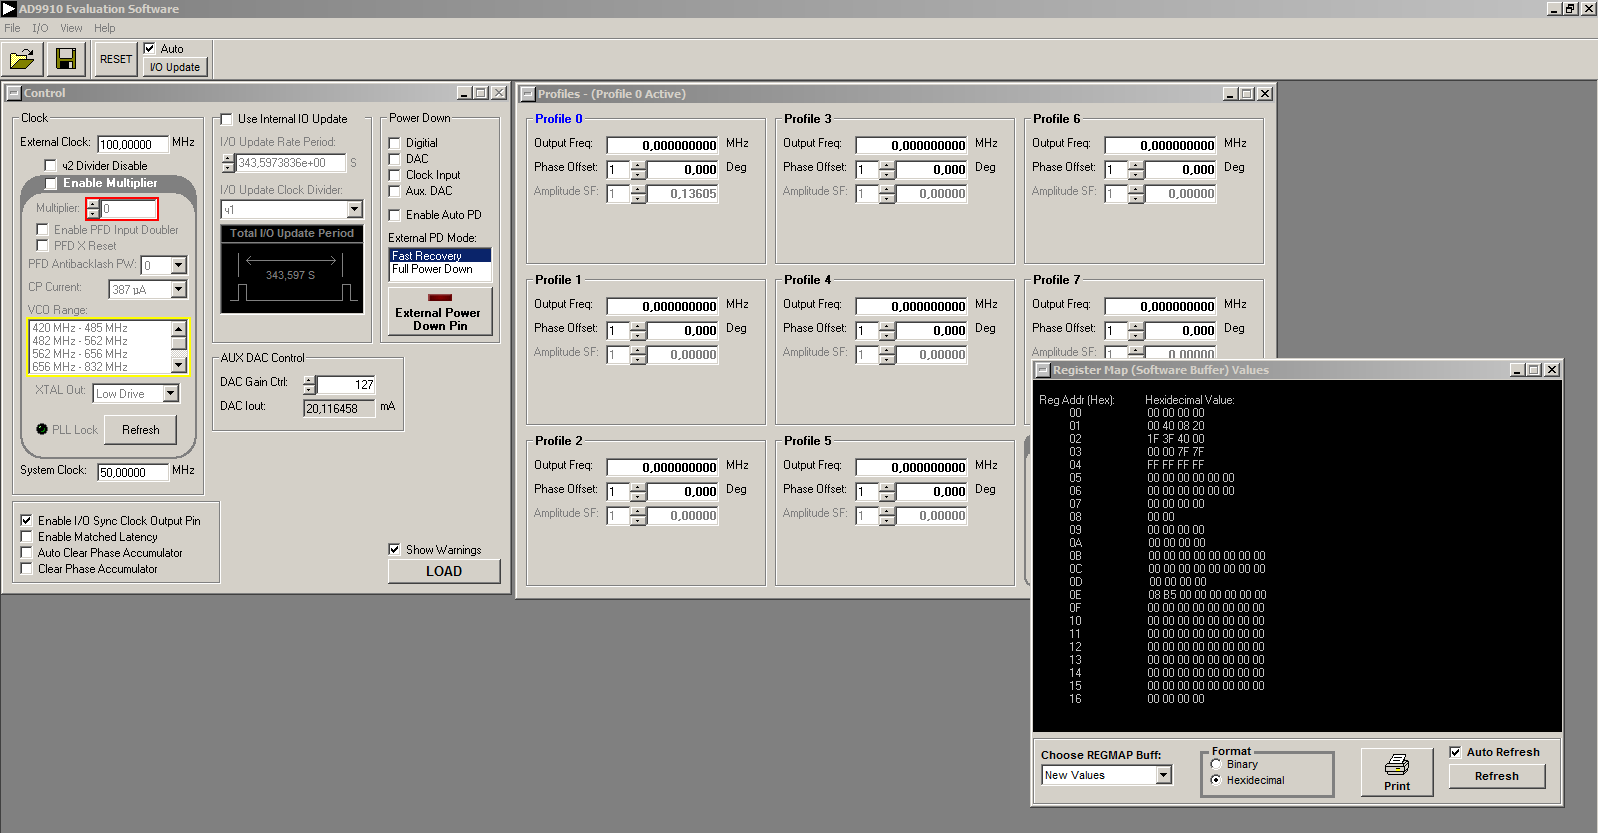
\includegraphics[scale=.25]{data/ad9910_evaluation_software.png}
\caption{Утилита управления синтезатором AD9910 с ПК.}
\label{fig:ad9910_evaluation_software}
\end{figure}
\end{gostfigure}

Всего синтезатор имеет 23 регистра с различной шириной, от 2 байт до 8 байт. В большинстве случаев, один бит регистра отвечает за включение/выключение определённой функции синтезатора, но есть некоторые регистры, которые отведены под хранение числовых значений, например регистры 15--22 используются для хранения восьми профилей генерируемой частоты. Полное описание полей регистров чипа AD9910 можно найти в источнике \cite{AD9910Datasheet}.

Управление синтезатором осуществляется при помощи SPI и множества выделенных под отдельные функции управляющих сигналов, схема подключений которых представлена на рисунке \ref{fig:wiring_diagram}. В режиме управления внешним микроконтроллером, встроенный микроконтроллер должен быть отключен путём перестановки перемычек на плате синтезатора.

В рамках одной SPI транзакции синтезатору сначала отправляется инструкция размером в один байт, где старший бит выбирает между режимом записи и режимом чтения, а пять младших битов определяют номер регистра. В режиме записи должны последовать {\em n} байт данных, где {\em n} --- ширина регистра, а в режиме чтения, наоборот, должно быть считано {\em n} байт данных.

Значения, записанные в регистры синтезатора, вступают в силу не сразу. Изначально они находятся в буфере ввода-вывода, и чтобы скопировать их в действующие регистры, нужно подать короткий сигнал высокого уровня на вход IO\_UPDATE, что далее по тексту называется ``Выполнить IO\_UPDATE.'' Перенос значений в действующие регистры также произойдёт в результате изменения состояния входов профилей, когда происходит выбор профиля, отличного от выбранного ранее.

\subsubsection{Формирование непрерывных сигналов}

Для начального запуска синтезатора под управлением внешнего микроконтроллера был использован подход с записью всех регистров эталонными значениями: благодаря утилите производителя было известно, какое в точности содержимое должно быть в каждом регистре синтезатора для получения непрерывного сигнала на некоторой частоте. Так как внутреннее состояние синтезатора представлено только его регистрами, можно перезаписать содержимое всех регистров этими заранее известными значениями, и, при прочих равных условиях, синтезатор должен начать генерировать сигнал на выходе. Технически, содержимое оперативной памяти тоже является внутренним состоянием синтезатора, но на данном этапе оперативная память не используется.

Было обнаружено, что отключение встроенного микроконтроллера приводит к переходу входов MASTER\_RESET и EXT\_PWD\_DOWN в неопределённое состояние, из-за чего синтезатор не работает. Добавление перемычек, подтягивающих эти входы к низкому уровню, разрешило проблему --- после записи известных значений в регистры синтезатора на выходе был получен сигнал. Переход от записи полностью фиксированных значений в регистры к программному изменению основных параметров сигнала стал следующим шагом.

% Реализовано в:
% - https://github.com/AXKuhta/stm32_ad9910/commit/272f2d1457d6abef2580f479caacd4918fd27638
% - https://github.com/AXKuhta/stm32_ad9910/commit/0c8fbba4f038878d401e76cec10e339cd68cf210

В AD9910 на сигнал влияют три основных параметра:

\begin{table}[H]
\centering
\caption{Параметры сигнала в AD9910}
\label{tab:signal_parameters}
\begin{tabular}{|p{4cm}|p{8cm}|}
\hline 
\textbf{Название} & \textbf{Пояснение} \\ 
\hline 
$FTW$ & 32-х битное значение частоты. \\ 
\hline
$POW$ & 16-ти битное значение сдвига фазы. \\
\hline
$ASF$ & 14-ти битное значение амплитуды. \\
\hline
\end{tabular} 
\end{table}

За выбор источника $FTW$, $POW$ и $ASF$ отвечает коммутатор шин, прямого контроля над которым нет и который автоматически выбирает один источник из набора активных источников на основе определённых аппаратно приоритетов. В конфигурации по умолчанию, частота и фаза берутся из регистров профилей, а амплитуда берётся из общего вторичного регистра. Чтобы включить индивидуальную амплитуду для каждого профиля, необходимо включить бит Enable Amplitude Scale from Single Tone Profiles, который выключен по умолчанию.

Ниже представлена структура полей одного профиля:

%
% Структура полей в регистрах профилей.
%
\begin{gostfigure}
\begin{figure}[H]
\centering
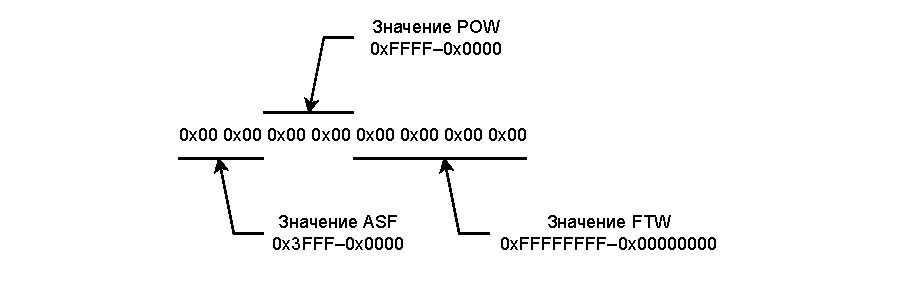
\includegraphics{data/single_tone_profile_register_layout.drawio.pdf}
\caption{Структура полей в регистрах профилей.}
\label{fig:single_tone_profile_register_layout}
\end{figure}
\end{gostfigure}

Для подачи сигналов на некоторой произвольной частоте необходимо вычислить значение $FTW$ по формуле $\lfloor a\frac{2^{32}}{b} + 0.5 \rfloor$, где $a$ --- требуемая частота в Гц, а $b$ --- тактовая частота синтезатора в Гц, затем вставить это значение в один из профилей. Также потребуется выставить значение амплитуды.

Эти операции реализованы в команде {\footnotesize\ttfamily{test\_tone [freq] [unit]}}, которая изменяет частоту и амплитуду одного из профилей в хранимой микроконтроллером копии регистров. Для активации изменений все регистры синтезатора перезаписываются обновлённым снимком регистров, после чего выполняется IO\_UPDATE и выбирается профиль с новыми значениями.

\subsubsection{Формирование коротких импульсов}

Для подачи импульсов вместо непрерывных сигналов необходимо реализовать прекращение и возобновление подачи сигналов. Прекращение сигнала можно получить двумя способами: отключение ЦАП или подача на ЦАП нулей. В AD9910 нет механизмов для отключения ЦАП отдельно от остальных частей синтезатора, так что единственным способом прервать подачу сигнала без частичного или полного отключения синтезатора является переход в такое состояние, когда на ЦАП по внутренней шине данных поступают только нули. Это  можно сделать при помощи применения нулевой амплитуды в блоке масштабирования амплитуды. В данном случае, на короткие импульсы можно смотреть как на частный случай амплитудной модуляции: амплитуда равна ненулевому значению внутри импульса, и нулю всё остальное время.

Технически, получить состояние, в котором на ЦАП поступают только нули, также можно при помощи удержания аккумулятора фазы в точке, где значение синусоиды равно нулю, но данный способ менее удобен, поскольку включение статического сброса фазы требует изменения регистров синтезатора и связанную с этим сравнительно длительную транзакцию по SPI, в то время, как применить нулевую амплитуду можно одним быстрым переключением профиля.

% Реализовано в:
% - https://github.com/AXKuhta/stm32_ad9910/commit/2e487a1fa9ddbbce861b1afd3613c8091fd185eb
В текущей реализации нулевой профиль зарезервирован под прекращение подачи сигнала и режим ожидания триггера. Для начала подачи сигнала происходит переключение на другой профиль с ненулевой амплитудой. Ранее, переключение профиля осуществлялось из контекста прерывания на микроконтроллере, с достаточно большим разбросом по времени. Позднее, для установки уровней на входах профилей был задействован DMA, что позволило уменьшить разброс.

В данном подходе присутствует проблема с непредсказуемой начальной фазой: включение профиля с нулевой амплитудой и нулевой частотой убирает сигнал с выхода и останавливает изменение значения в аккумуляторе фазы, но не сбрасывает его. В этом кроется проблема: в момент начала следующего импульса старое значение фазы приведёт к началу сигнала со значения синусоиды в произвольной точке, а не в нуле, что выглядит на осциллографе как резкий прыжок или резкий провал в начале синусоидальной волны. Из непредсказуемой начальной фазы также следует непредсказуемость фазы во всех остальных точках сигнала; иными словами, положение пиков в синусоидальной волне на протяжении всего сигнала различается между запусками. Данная проблема не мешает использованию калибратора для снятия АЧХ, но исключает возможность снятия ФЧХ.

На рисунке ниже представлено наглядное изображение проблемы: слева изображено начало синусоидального сигнала с нулевой фазой, а справа начало синусоидального сигнала со случайной фазой.

%
% Нулевая начальная фаза и случайная начальная фаза.
%
\begin{gostfigure}
\begin{figure}[H]
\centering
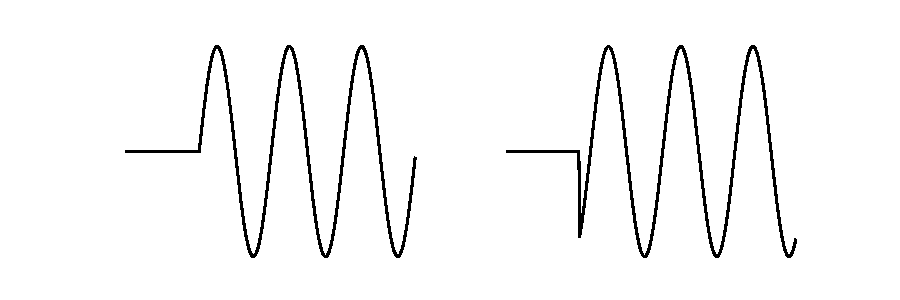
\includegraphics{data/random_start_phase.pdf}
\caption{Нулевая начальная фаза и случайная начальная фаза.}
\label{fig:random_start_phase}
\end{figure}
\end{gostfigure}

% https://tex.stackexchange.com/questions/168430/xelatex-polyglossia-hyphenation
Проблема с непредсказуемой начальной фазой решается использованием статического сброса аккумулятора фазы: при включении бита Clear phase accumulator, аккумулятор фазы принудительно удерживается в сброшенном состоянии, т.е. всегда равен нулю и не увеличивается. Чтобы начать подачу сигнала из этого состояния, нужно выключить статический сброс до начала подачи следующего сигнала и применить изменения. После выключения статического сброса, если выбран профиль с нулевой частотой, то значение аккумулятора не начнёт увеличиваться и по шине данных на ЦАП продолжат поступать нули. Затем, когда будет включен профиль с ненулевой частотой, значение аккумулятора фазы начнёт расти с нуля и на выходе получится сигнал с предсказуемой начальной фазой.

Ниже представлена диаграмма, на которой изображена итоговая схема подачи коротких импульсов:

%
% Процедура подачи коротких импульсов.
%
\begin{gostfigure}
\begin{figure}[H]
\centering
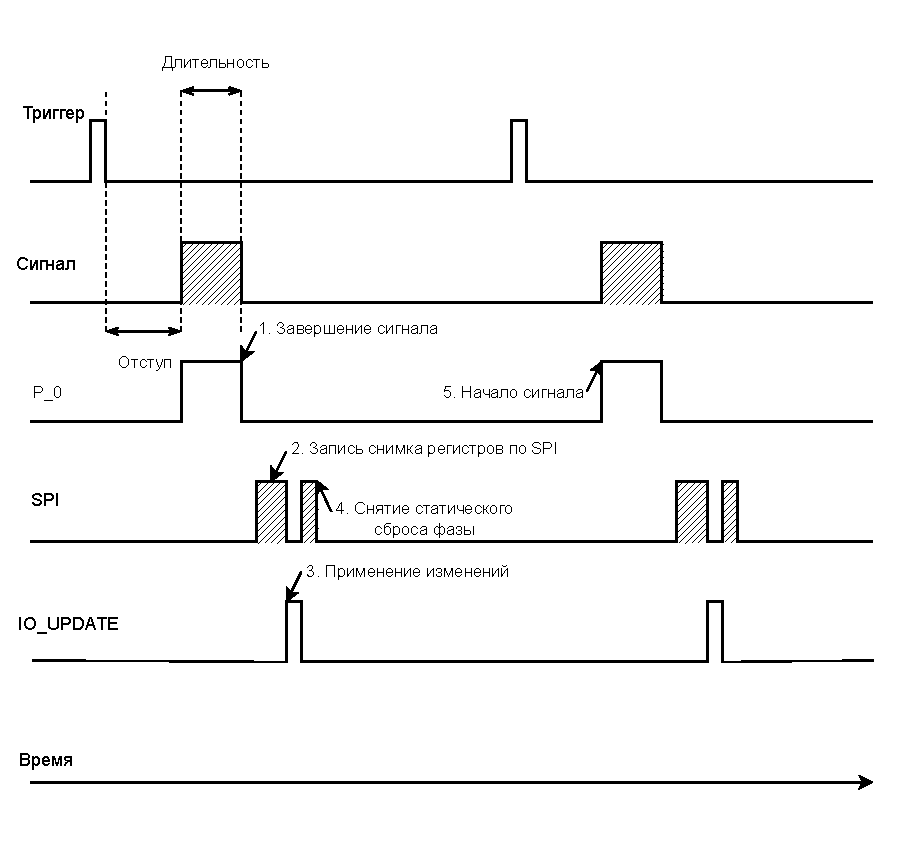
\includegraphics{data/detailed_timing_diagram.drawio.pdf}
\caption{Процедура подачи коротких импульсов.}
\label{fig:detailed_timing_diagram}
\end{figure}
\end{gostfigure}

Показано переключение только одного из входов профилей, поскольку остальные не задействованы и сохраняют низкий уровень. Данная схема верна для сигналов на фиксированной частоте, для ЛЧМ сигналов и для сигналов с модуляцией при помощи оперативной памяти AD9910, но не для сигналов с модуляцией при помощи профилей, где уровни на входах P\_x изменяются в процессе подачи сигнала.

\subsubsection{Использование AD9910 для ЛЧМ сигналов}

Для реализации линейной частотной модуляции используется блок \textenglish{Digital Ramp Generator} (DRG) в AD9910. Блок DRG является 32-х битным счётчиком, выходное значение которого можно использовать в качестве параметра частоты, амплитуды или фазы сигнала, хотя в случае с амплитудой и фазой задействованы только 16 и 14 младших бит соответственно.

Управление блоком DRG осуществляется через шесть параметров в регистрах:

\begin{itemize}
	\item Величина инкремента.
	\item Величина декремента.
	\item Делитель частоты инкрементов.
	\item Делитель частоты декрементов.
	\item Нижняя граница значения.
	\item Верхняя граница значения.
\end{itemize}

Выбор между использованием значений инкремента и декремента осуществляется через уровень на входе DR\_CTL. Исходя из активного значения делителя частоты, DRG может делать отсчёты со скоростью от 250 МГц до $\frac{250}{65535}$ МГц. Количество инкрементов на протяжении одного сигнала можно выразить как $\text{steps} = d\frac{250 \text{ МГц}}{b}$, где $d$ --- длительность в секундах, а $b$ --- делитель частоты инкрементов. Нужно обратить внимание, что последний инкремент будет сделан в момент окончания сигнала, следовательно, будет сделано только $\text{steps}-1$ видимых инкрементов.

При использовании DRG для ЛЧМ сигналов с нарастающей частотой, полосу сигнала (то есть разницу между начальной и конечной частотой) можно выразить как $\text{band} = a\frac{1 \text{ ГГц}}{2^{32}} \bigl( \text{steps} - 1\bigr)$, где $a$ --- величина инкремента. Начальная частота задаётся значением в регистре нижней границы.

Команды для режимов работы с ЛЧМ сигналами в текстовом интерфейсе калибратора принимают в качестве аргументов значения $a$ и $b$, длительность и центральную частоту $f_c$. Начальная и конечная частоты вычисляются автоматически как $f_1 = f_c - \frac{\text{band}}{2}, f_2 = f_c + \frac{\text{band}}{2}$.

ЛЧМ сигналы с убывающей частотой являются особым случаем из-за того, что сброс счётчика возможен только на нижнюю границу, а нижняя граница должна быть меньше верхней границы. Данную проблему удалось преодолеть использованием зеркальных частот, которые получаются при значениях $FTW > 2^{31}$; смысл таких значений $FTW$ меняется, и большие значения соответствуют меньшим частотам, что позволяет использовать меньшее значение, соответствующее большей начальной частоте, в качестве нижней границы, и наоборот, использовать значение с меньшей частотой в качестве верхней границы. Главной особенностью такого режима работы синтезатора является то, по своему наблюдаемому поведению аккумулятор фазы становится обратным счётчиком, и генерация синусоиды начинается с конца, что выглядит на осциллографе как повёрнутая на 180 градусов фаза, что, к счастью, легко компенсируется.

\subsubsection{Использование оперативной памяти AD9910}

Встроенная оперативная память AD9910 способна вместить 1024 32-х битных слова и может использоваться в качестве источника значения частоты, амплитуды, сдвига фазы, либо амплитуды и фазы одновременно, что называется полярным режимом. В режиме источника частоты используются все 32 бита в каждом слове, а в режиме источника фазы или источника амплитуды используются старшие 16 или 14 бит соответственно. В полярном режиме старшие 16 бит отвечают за фазу и последующие 14 бит отвечают за амплитуду, а два оставшихся бита не используются.

За выбор адреса в памяти отвечает стейт-машина, у которой есть два основных режима работы: воспроизведение и чтение либо запись. В режиме воспроизведения, в зависимости от настроек, стейт-машина памяти может перемещаться по адресам следующими способами:

\begin{itemize}
	\item Удерживать начальный адрес.
	\item Пройти до конца.
	\item Пройти до конца и обратно.
	\item Циклично ходить до конца.
	\item Циклично ходить до конца и обратно.
\end{itemize}

Указание начального и конечного адреса для воспроизведения осуществляется при помощи регистров профилей, содержимое которых приобретает альтернативный порядок и смысл. Когда используется оперативная память, каждый профиль, помимо начального и конечного адреса, задаёт режим перемещения по адресам и делитель частоты шагов при воспроизведении, о котором проще думать, как о длительности одного элемента. На полной тактовой частоте, максимальная длительность одного элемента в памяти составляет $65535\times4$ нс $=$ 262.14 мкс. Изменение профиля приводит к сбросу стейт-машины и началу воспроизведения заново.

Чтение и запись оперативной памяти по SPI выполняется пока воспроизведение из оперативной памяти выключено, то есть бит RAM Enable равен нулю. Начальный и конечный адрес для операций чтения и записи берутся из регистров профилей, в связи с чем возникает интересная особенность: пока воспроизведение из памяти выключено, используется значение $FTW$ из регистров профилей, а поля начального и конечного адреса памяти пересекаются с полем $FTW$. Для избежания возникновения неожиданных сигналов на выходе синтезатора после установки начального/конечного адреса памяти необходимо заранее включить статический сброс фазы или применить нулевое значение амплитуды.

После установки требуемого начального и конечного адреса в регистре любого профиля и выбора соответствующего профиля (или применения изменений, если профиль уже выбран), по интерфейсу SPI производится череда транзакций для считывания или записи одного слова, причём общее количество транзакций должно быть равно разнице между конечным адресом и начальным адресом. Нужно иметь в виду, что при операциях чтения или записи, счётчик адреса оперативной памяти почему-то работает в обратном режиме, начиная отсчёт с конечного адреса и отсчитывая до начального.

Имея возможность автономно изменять параметры сигнала в зависимости от времени, не полагаясь на медленный внешний микроконтроллер, блок оперативной памяти полезен не только для модуляции, но и для создания точных по длительности сигналов в целом, что было применено для улучшения сигналов с фиксированной частотой и ЛЧМ сигналов относительно их изначальной реализации. Ранее, для завершения подобных сигналов использовалось переключение профилей со стороны микроконтроллера, что вносило примерно 25 нс разброса в общую длительность. Данный разброс удалось полностью исключить путём использования оперативной памяти для точного по времени обрыва сигнала посредством установки нулевой амплитуды.

При использовании DRG в сочетании с оперативной памятью была встречена проблема с непроизвольным смещением фазы сигнала в зависимости от начальной частоты. Причина крылась в том, что значения от DRG поступают на ядро DDS с меньшей задержкой по сравнению с оперативной памятью, даже когда включен режим Matched Latency; задержка составляет 106 тактов для амплитуды, и 91 такт для частоты. Значение $FTW$ начинает поступать аккумулятору фазы существенно раньше, чем ненулевое значение $ASF$ начинает поступать блоку масштабирования амплитуды, что приводит к потере начальной части синусоиды.

Проблема была решена механизмом компенсации, который сдвигает начальную фазу таким образом, чтобы по прошествии 20 тактов получилась нулевая фаза. Было установлено, что вычет прогнозируемой спустя 15 тактов фазы (предполагаемая на основе значений из даташита разница задержек) не позволяет полностью избавиться от проблемы.

\subsection{Результаты}

Калибратор испытан в лабораторных и реальных условиях: проверена интеграция с упрощённой копией регистрирующего оборудования ИРНР, и с полным вариантом, расположенным непосредственно на радаре. Получено множество записей сигналов в разных режимах работы калибратора, но наиболее интересным результатом являются графики АЧХ во всём рабочем диапазоне частот ИРНР, которые были получены отдельно для одного из выносных устройств приёма (ВУП), и для приёмного тракта в целом.

Для измерения АЧХ ВУП 2 в лабораторных условиях использовалась цепочка из калибратора, разветвителя на два канала, ВУП и регистрирующего устройства (DDC). Калибратор использовался для подачи коротких ЛЧМ импульсов с полосой примерно 4 МГц на разной центральной частоте: 156 МГц, 158 МГц, 160 МГц. Эти сигналы покрывают весь рабочий диапазон частот ИРНР и для каждой частоты было записано большое количество импульсов, что даёт возможность использовать усреднение. Затем, ВУП был исключен из схемы и схожий набор сигналов был записан, используя только калибратор, разветвитель и DDC.

Построена диаграмма примерной АЧХ ВУП 2 (Рисунок \ref{fig:vup2}) в отдельности от других компонентов, полученная в результате деления усреднённой амплитуды сигналов с ВУП на усреднённую амплитуду эквивалентных сигналов без ВУП. Поскольку график составлен из трёх отдельных сигналов, разделённых на два канала, получившаяся диаграмма содержит шесть линий разного цвета, которые образуют две кривые --- АЧХ двух каналов ВУП.

%
% АЧХ ВУП 2
%
\begin{gostfigure}
\begin{figure}[H]
\centering
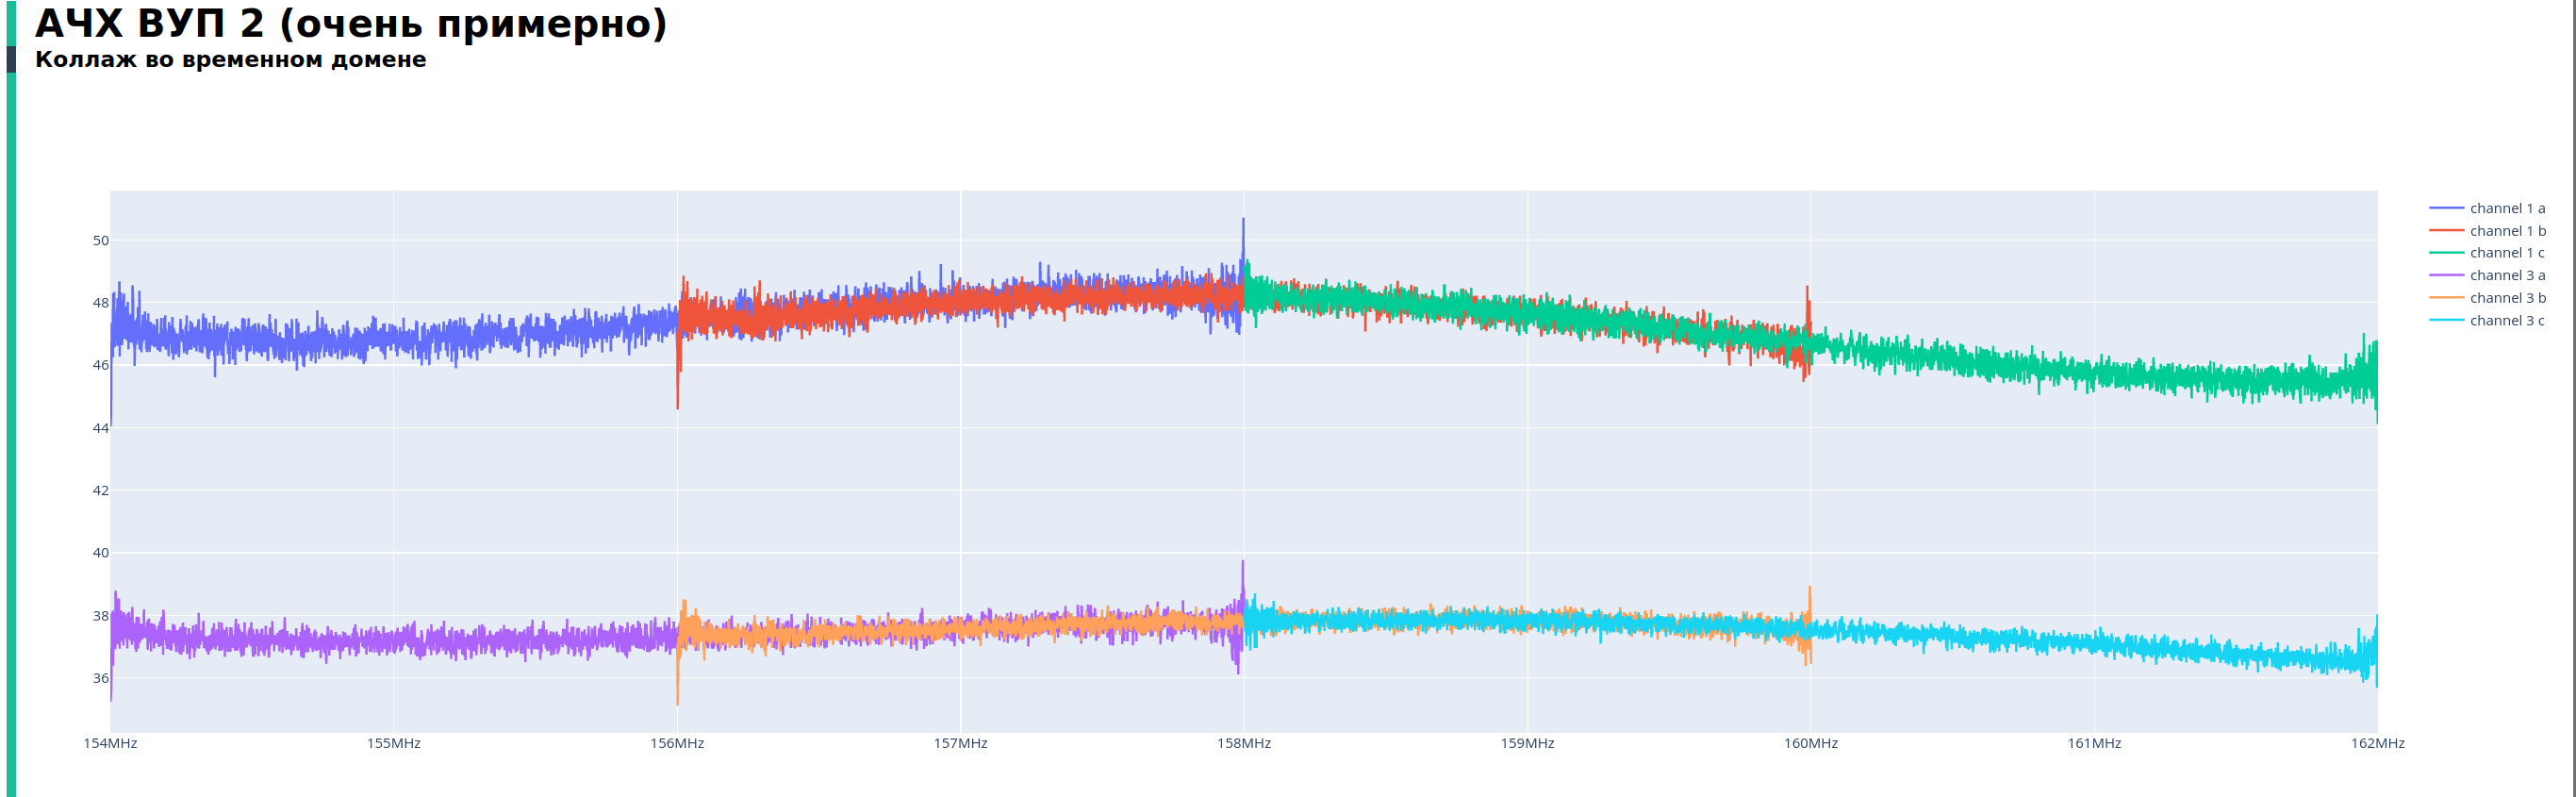
\includegraphics[scale=.15]{data/vup2.png}
\caption{АЧХ ВУП 2.}
\label{fig:vup2}
\end{figure}
\end{gostfigure}

Похожие измерения были выполнены в реальных условиях с приёмным трактом ИРНР, но без исключения отдельных компонентов. Используя данные из экспериментов в лаборатории для удаления вносимой калибратором и DDC составляющей, был получен график АЧХ для всего приёмного тракта (Рисунок \ref{fig:vup1etc}).

%
% АЧХ ВУП 2
%
\begin{gostfigure}
\begin{figure}[H]
\centering
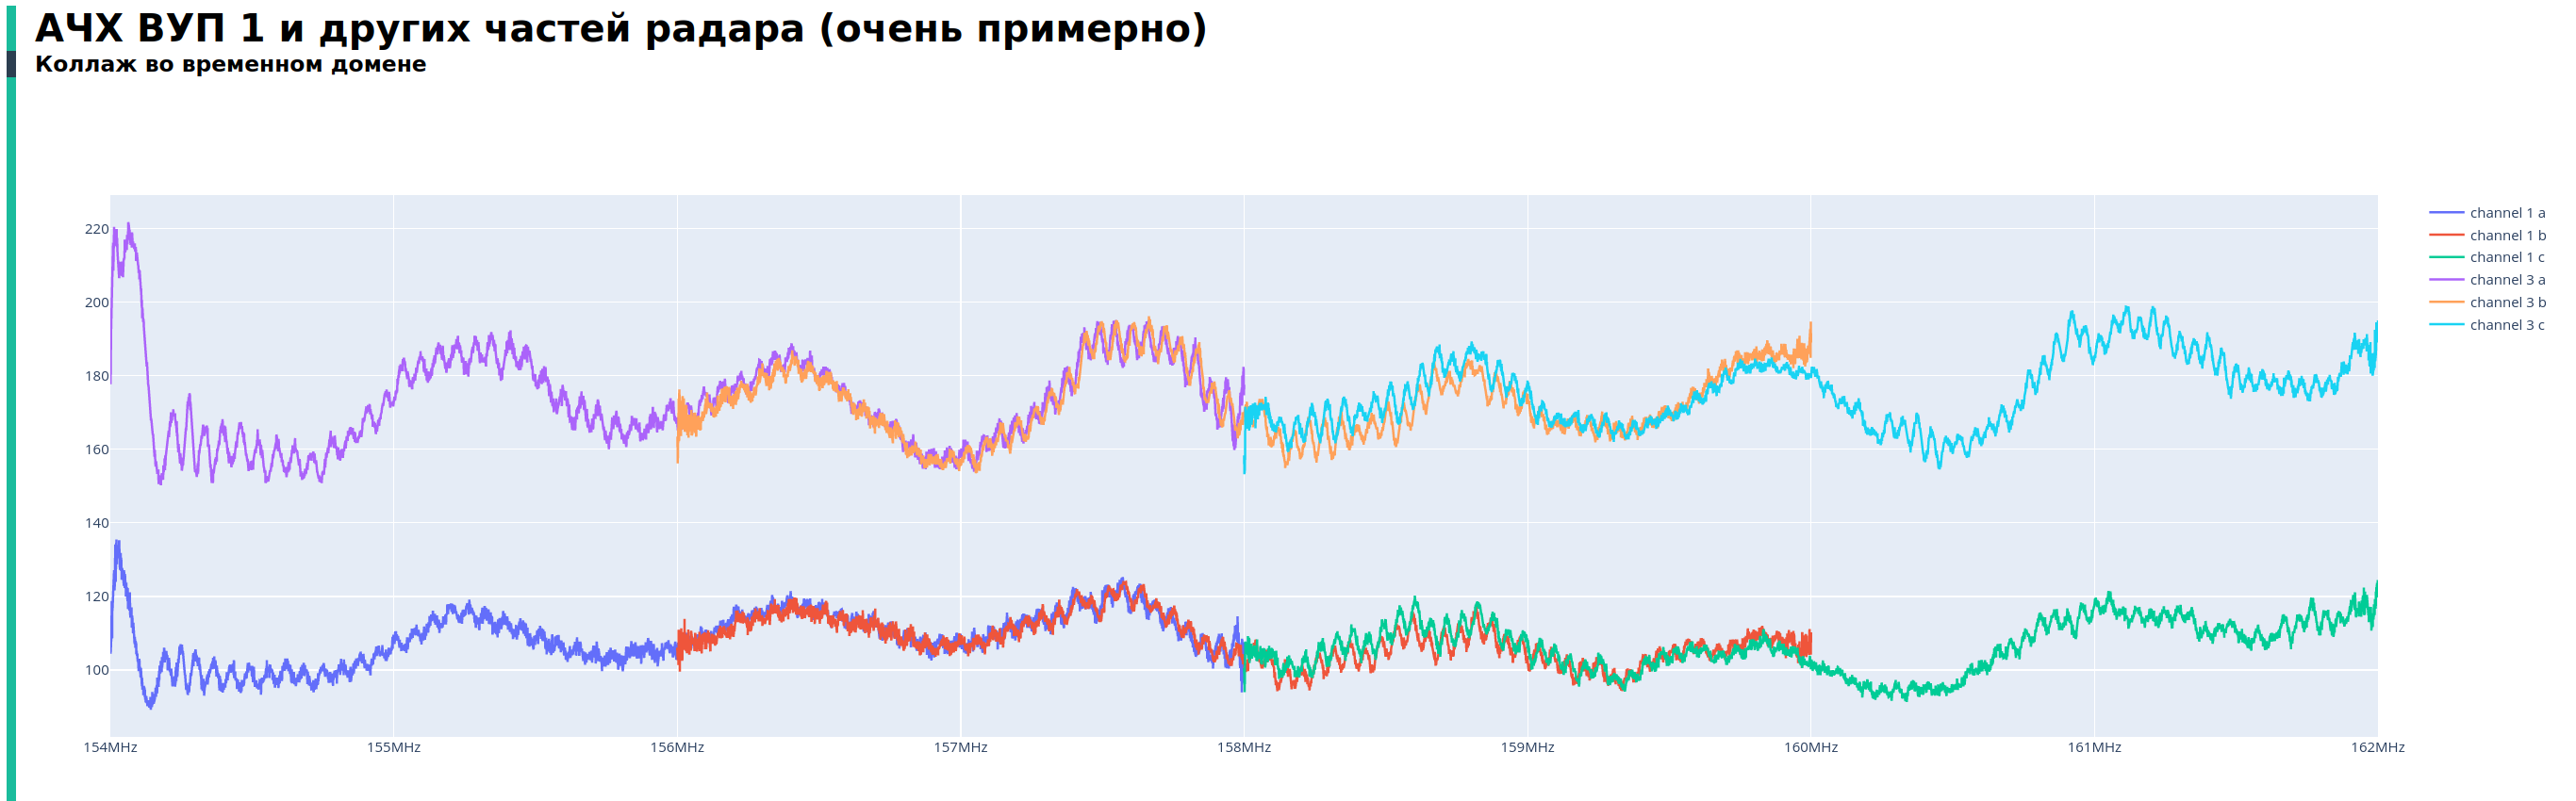
\includegraphics[scale=.15]{data/vup1etc.png}
\caption{АЧХ ВУП 1 и других частей приёмного тракта.}
\label{fig:vup1etc}
\end{figure}
\end{gostfigure}

Видно, что АЧХ всей системы обладает существенно более сложной формой. Установление причин такой сложной формы является темой для будущего исследования.


\section*{ЗАКЛЮЧЕНИЕ}

Разработан макет калибратора и встроенное ПО, которое реализует основные режимы работы (Непрерывные сигналы, короткие импульсы на фиксированной частоте, ЛЧМ импульсы, импульсы с фазовой манипуляцией.) и управление с ПК по Ethernet и USB при помощи текстового интерфейса.

Калибратор испытан в лабораторных и реальных условиях, проверена интеграция со штатным регистрирующим оборудованием ИРНР и получены первые результаты. Наличие подобного устройства делает возможным исследование характеристик антенно-фидерного и приёмного тракта ИРНР как единой системы, в сквозном режиме.

Целесообразна доработка калибратора. Дальнейшие направления работы включают:

\begin{itemize}
	\item Дополнительные режимы работы, которые более точно повторяют сигналы, используемые ИРНР во время наблюдений.
	\item Разработку графического интерфейса GUI для управления калибратором.
	\item Повышение точности отсчёта времени задержки и длительности сигналов.
	\item В перспективе, реализацию автоматической калибровки приёмного тракта ИРНР.
\end{itemize}

% Список литературы.
\begin{thebibliography}{11}
\bibitem{DDSIntro} Компоненты и технологии, Всё о синтезаторах DDS
https://web.archive.org/web/http://www.kit-e.ru/assets/files/pdf/ \\
2005\_01\_28.pdf
\bibitem{DDSTutorial} A Technical Tutorial
on Digital Signal Synthesis https://www.ieee.li/pdf/essay/dds.pdf
\bibitem{STM32F746Datasheet} STMicroelectronics, STM32F746xx Datasheet
\bibitem{NucleoDatasheet} STMicroelectronics, STM32 Nucleo-144 boards (MB1137)
\bibitem{AD9910Datasheet} Analog Devices, AD9910 Datasheet
\bibitem{Kushnarev} Кушнарев Д.С., Лебедев В.П., Хахинов В.В., Евстифеев С.Е., Заруднев В.Е. Модернизация Иркутского радара некогерентного рассеяния. Солнечно-земная физика. 2017. Т. 3, № 3. С. 88-94.
\end{thebibliography}

\appendix

\begin{gostappendix}{Схема подключений}
\renewcommand{\thesection}{\Alph{section}}
\renewcommand{\thesubsection}{subsection}
\setcounter{section}{1}
\setcounter{figure}{0}
\begin{gostfigure}
\begin{figure}[H]
\centering
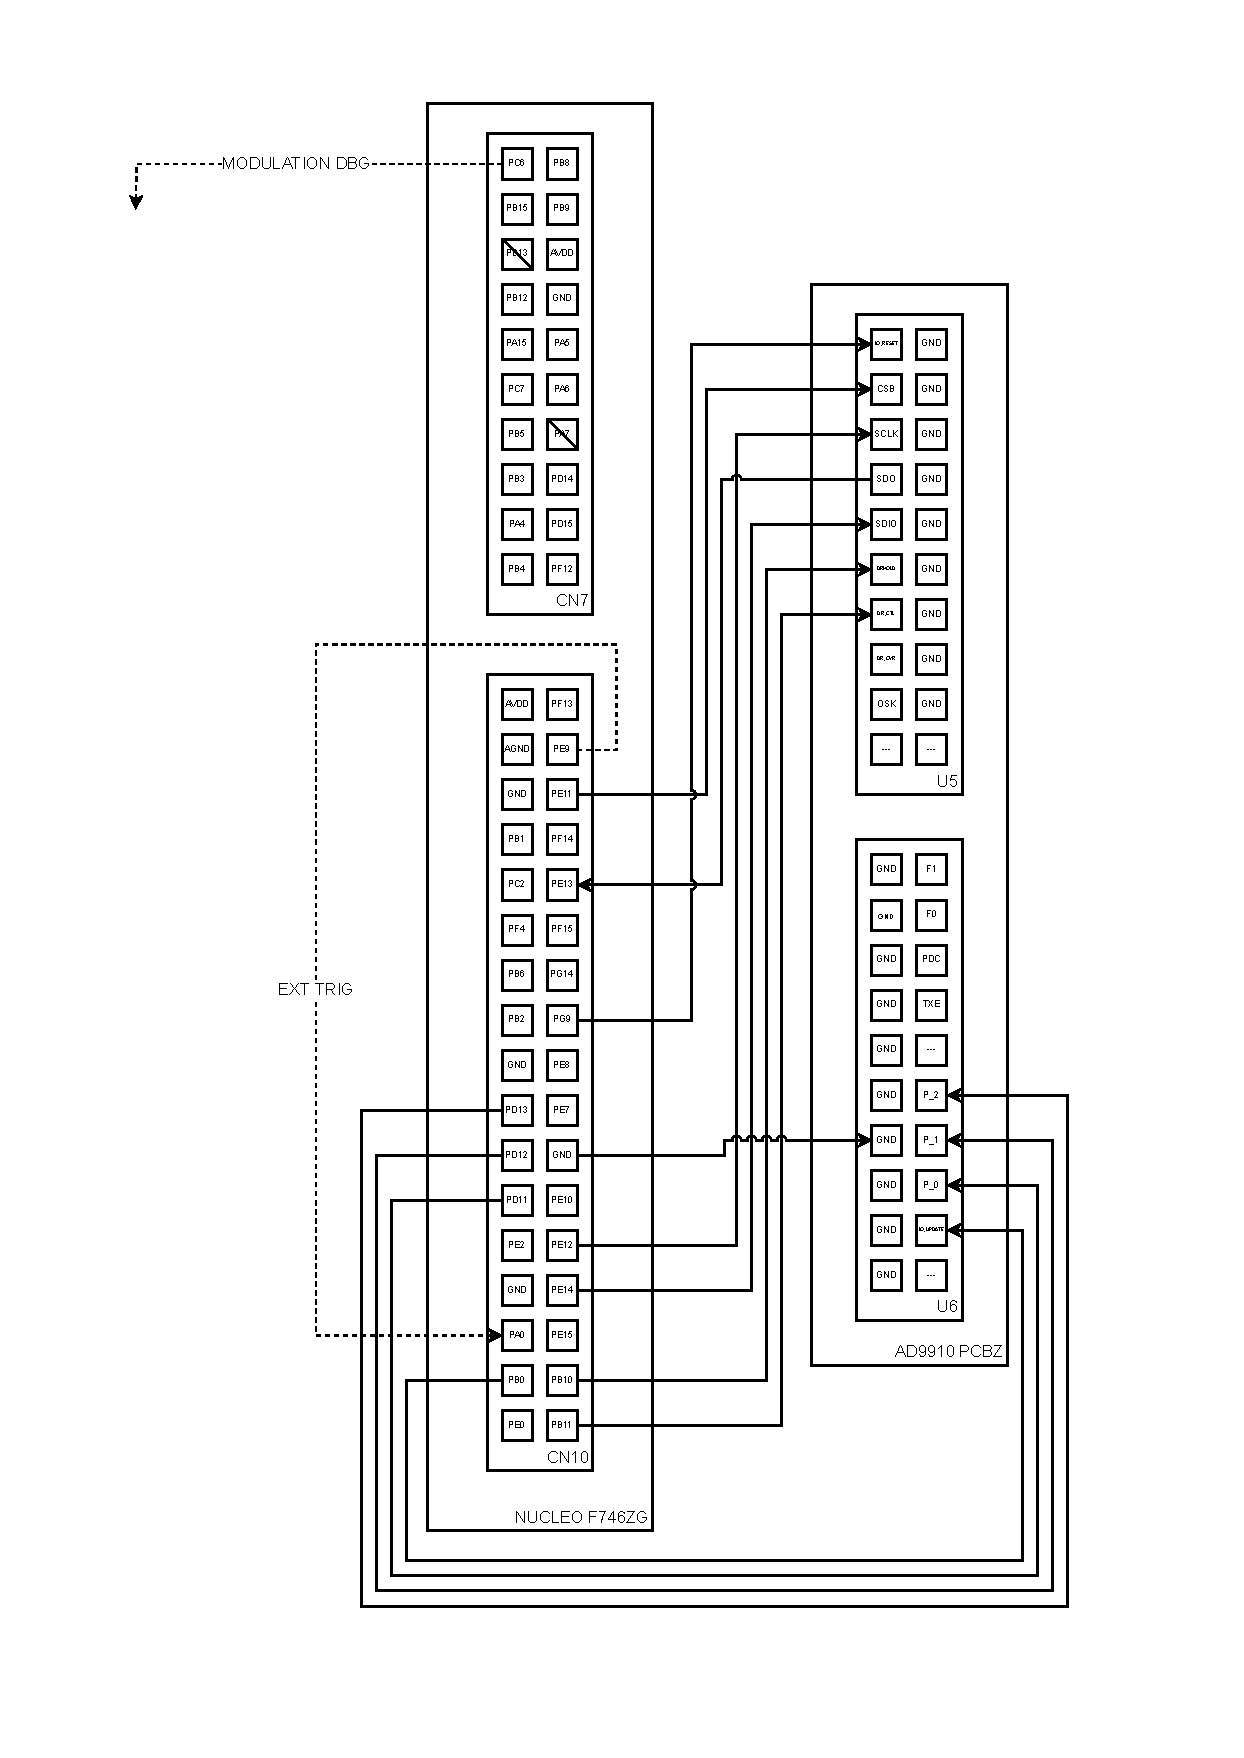
\includegraphics[scale=.75]{data/wiring_diagram.drawio.pdf}
\caption{Схема подключений.}
\label{fig:wiring_diagram}
\end{figure}
\end{gostfigure}
\end{gostappendix}

\end{document}
